
The effect of the quark-gluon sample selection on the sensitivity of the resonance search in the 
dijet mass is evaluated using a toy-MC simulation. The background is modelled using the simulation of \QCD\
jet production (Sec.~\ref{qcdsamps}) created using  \Pythia8. The simulation data split into \QQ, \QG\ and \GG\
subsamples using Eqs.~\ref{eq:QGselect} where \nqg\ is set using \ref{eq:nqg2} as shown 
in Fig.~\ref{fig:pythia_qg_selection}(b). To remove statistical fluctuations the mass distributions are fit to
\begin{equation}
f_i = \int_{m_a}^{m_b} p_0 \left(1 -x \right)^{p_1} x^{p_2 + p_3 ln(x) + p_4 \ln(x)^2  } dx
\label{eq:bf}
\end{equation}
where $f_i$ is the fit to bin $i$, $m_a$ and $m_B$ are the upper and lower bin edges, and $p_i$ are the fit parameters. 
The resulting distributions are normalised to the number of events in the 2015/16 resonance data set 
and used to generate data-like distributions with Poisson distributed random numbers (a pseudo-experiment). 

\textit{\color{red} Morphed signal shape.. } \ldots

For a given \qstar\ mass point each pseudo-experiment is fit with a background plus a morphed signal line shape. 
The background fit function is Eq.~\ref{eq:bf} and the signal is given by the morphed signal shape which has
been normalised to one. Expected 95\% confidence limits are determined for mass points from 2 to 6.5\,TeV in 0.5\,TeV
steps for the complete sample, the \QQ, \QG, and the \GG\ samples and for a combined fit of the \QQ, \QG\ 
and the \GG\ samples where 
\begin{linenomath}
\begin{align}
F_{\mathrm{sig}} + F_{\mathrm{bg}} ={}&  f_{QQ} N_X S_{QQ}(x) + B_{QQ}(x)  \nonumber \\
								   +{}&  f_{QG} N_X S_{QG}(x) + B_{QG}(x) \nonumber \\
								   +{}&  (1 - f_{QQ} -f_{QG})   N_X S_{QG}(x) + B_{QG}(x) 
\end{align}
\end{linenomath}
where $F_{\mathrm{sig}}$ and $F_{\mathrm{bg}}$ are the signal and background fits, $f_{QQ}$ ($f_{QG}$) is the 
fraction of the \qstar\ signal in the \QQ\ (\QG ) sub-sample given in Table~\ref{table:qstar_fractions}, $S_{QQ}$ 
($S_{QG}$, $S_{GG}$) 
are the morphed signal shapes, $B_{QQ}$ ($B_{QG}$, $B_{GG}$) are the independently fitted background functions  (Eq.~\ref{eq:bf}) and
$N_X$ is the fitted number of signal events. 

%Expected 95\% upper limits are calculated using a profile likelihood method, where the nuisance parameters are allowed 
%to float while the signal yield is scanned upward. 
%The 95\% upper limit is defined as the number of events 
%N such that 95\% of the resulting cumulative probability distribution lies below this value.
Expected 95\% upper limits are calculated using a profile likelihood method, where the nuisance parameters are allowed 
to float while the signal yield is scanned upward.  The 95\% upper limit is defined as the number of events 
N such that LLH(N) = LLH(base) + 1.92, approximately $2\sigma$ worse than the base case. For positive signals, 
LLH(Base) is the likelihood of the best-fit signal.  Otherwise, it is the likelihood corresponding to zero signal 
events. The expected upper limit is obtained by running the limit-setting procedure over the same pseudo-experiments 
as described above. The central value of the expected limit is taken to be the median of the pseudo-experiment 
distribution. The 1 and 2 sigma bands are taken to be median $\pm$ 34\% and median $\pm$ 47.5\% respectively.

The resulting limits for a \qstar model are given in Table~\ref{table:qstar_explimits} and shown in Fig.~\ref{fig:toyMCExpectedLimitsqstar}.
Combining the \QQ\ and \QG\ samples at 6.5\,TeV improves the limit on the cross section by a factor of approximately 7.


\begin{landscape}
\begin{table}[h]
	\centering 
		\caption{The expected 95\% upper limits for a sample the same size as the  2015 \& 16 data  determined 
		using a Toy-MC for the total sample (\JJ) the \QQ, \QG, and \GG\ sub-samples and the combined fit os the 
		sub-samples.
		\label{table:qstar_explimits}}
	\begin{tabular}{SSSSSS}
	\toprule
\qstar\ Mass (TeV) & \multicolumn{1}{c}{\JJ\ (pb)} &  \multicolumn{1}{c}{\QQ, \QG\ and \GG\  (pb)}  &  \multicolumn{1}{c}{\QQ\ (pb)} & \multicolumn{1}{c}{\QG\ (pb)} & \multicolumn{1}{c}{\GG\ (pb)} \\
\midrule 
2   & 6.94E-02 & 7.09E-02 & 2.94E-02 & 1.15E-01 & 1.63E-01 \\
2.5 & 3.87E-02 & 3.80E-02 & 2.88E-02 & 5.84E-02 & 5.83E-02 \\
3   & 2.11E-02 & 2.02E-02 & 2.00E-02 & 2.84E-02 & 2.23E-02 \\
3.5 & 1.13E-02 & 1.12E-02 & 1.31E-02 & 1.47E-02 & 9.80E-03 \\
4   & 7.14E-03 & 6.89E-03 & 9.16E-03 & 7.79E-03 & 5.78E-03 \\
4.5 & 4.31E-03 & 4.18E-03 & 6.35E-03 & 5.19E-03 & 3.22E-03 \\
5   & 2.84E-03 & 2.54E-03 & 4.35E-03 & 3.31E-03 & 2.35E-03 \\
5.5 & 1.89E-03 & 1.56E-03 & 3.01E-03 & 2.20E-03 & 1.87E-03 \\
6   & 1.35E-03 & 1.02E-03 & 2.14E-03 & 1.65E-03 & 1.97E-03 \\
6.5 & 9.77E-04 & 7.72E-04 & 1.62E-03 & 1.36E-03 & 2.13E-03 \\
7   & 7.46E-04 & 5.83E-04 & 1.23E-03 & 1.46E-03 & 1.99E-03 \\
\bottomrule
\end{tabular}
\end{table}
\end{landscape}


\begin{figure}[p]
 \centering

 \subfigure[JJ] {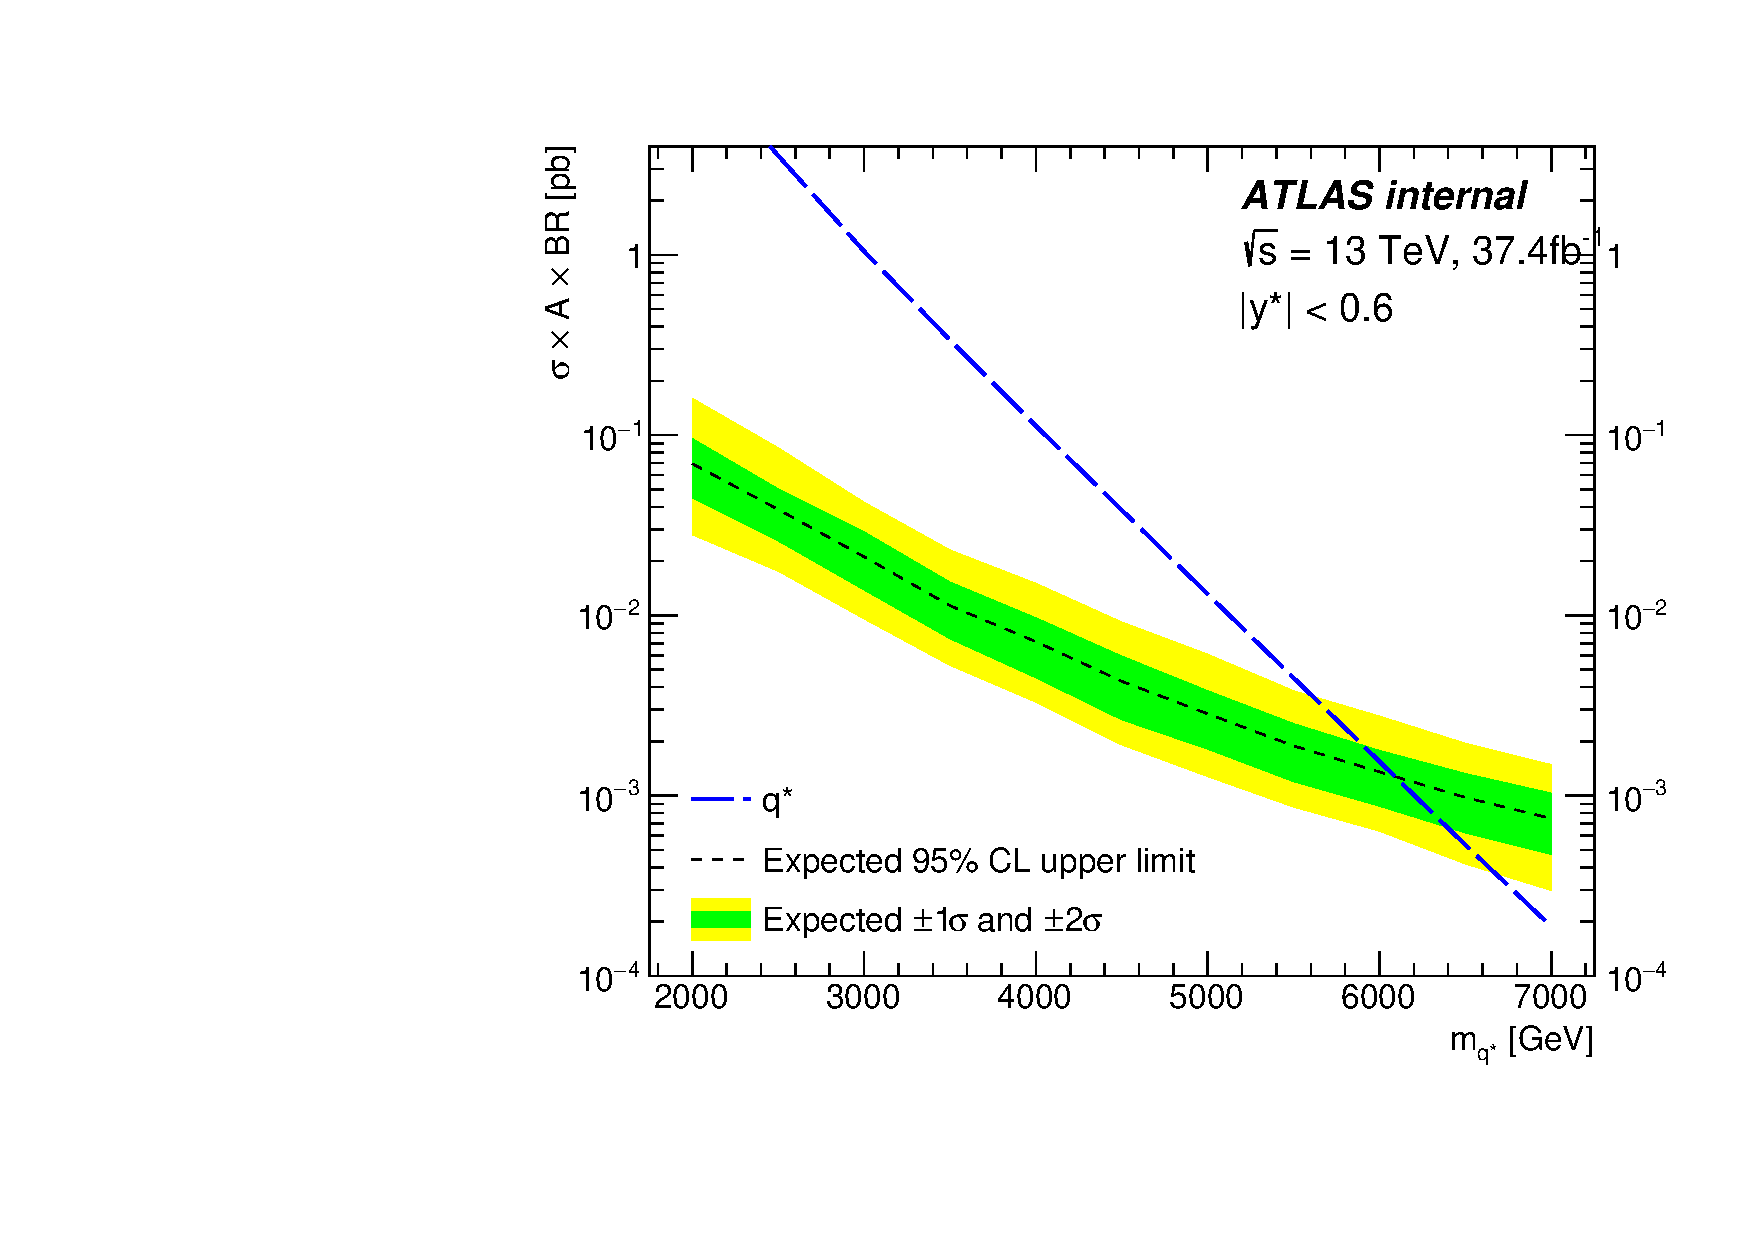
\includegraphics[width=0.475\textwidth] {figures/tagging/brazil-qStarMorphSingleJJUpdated.pdf}}
 \subfigure[\QQ\ \& \QG] {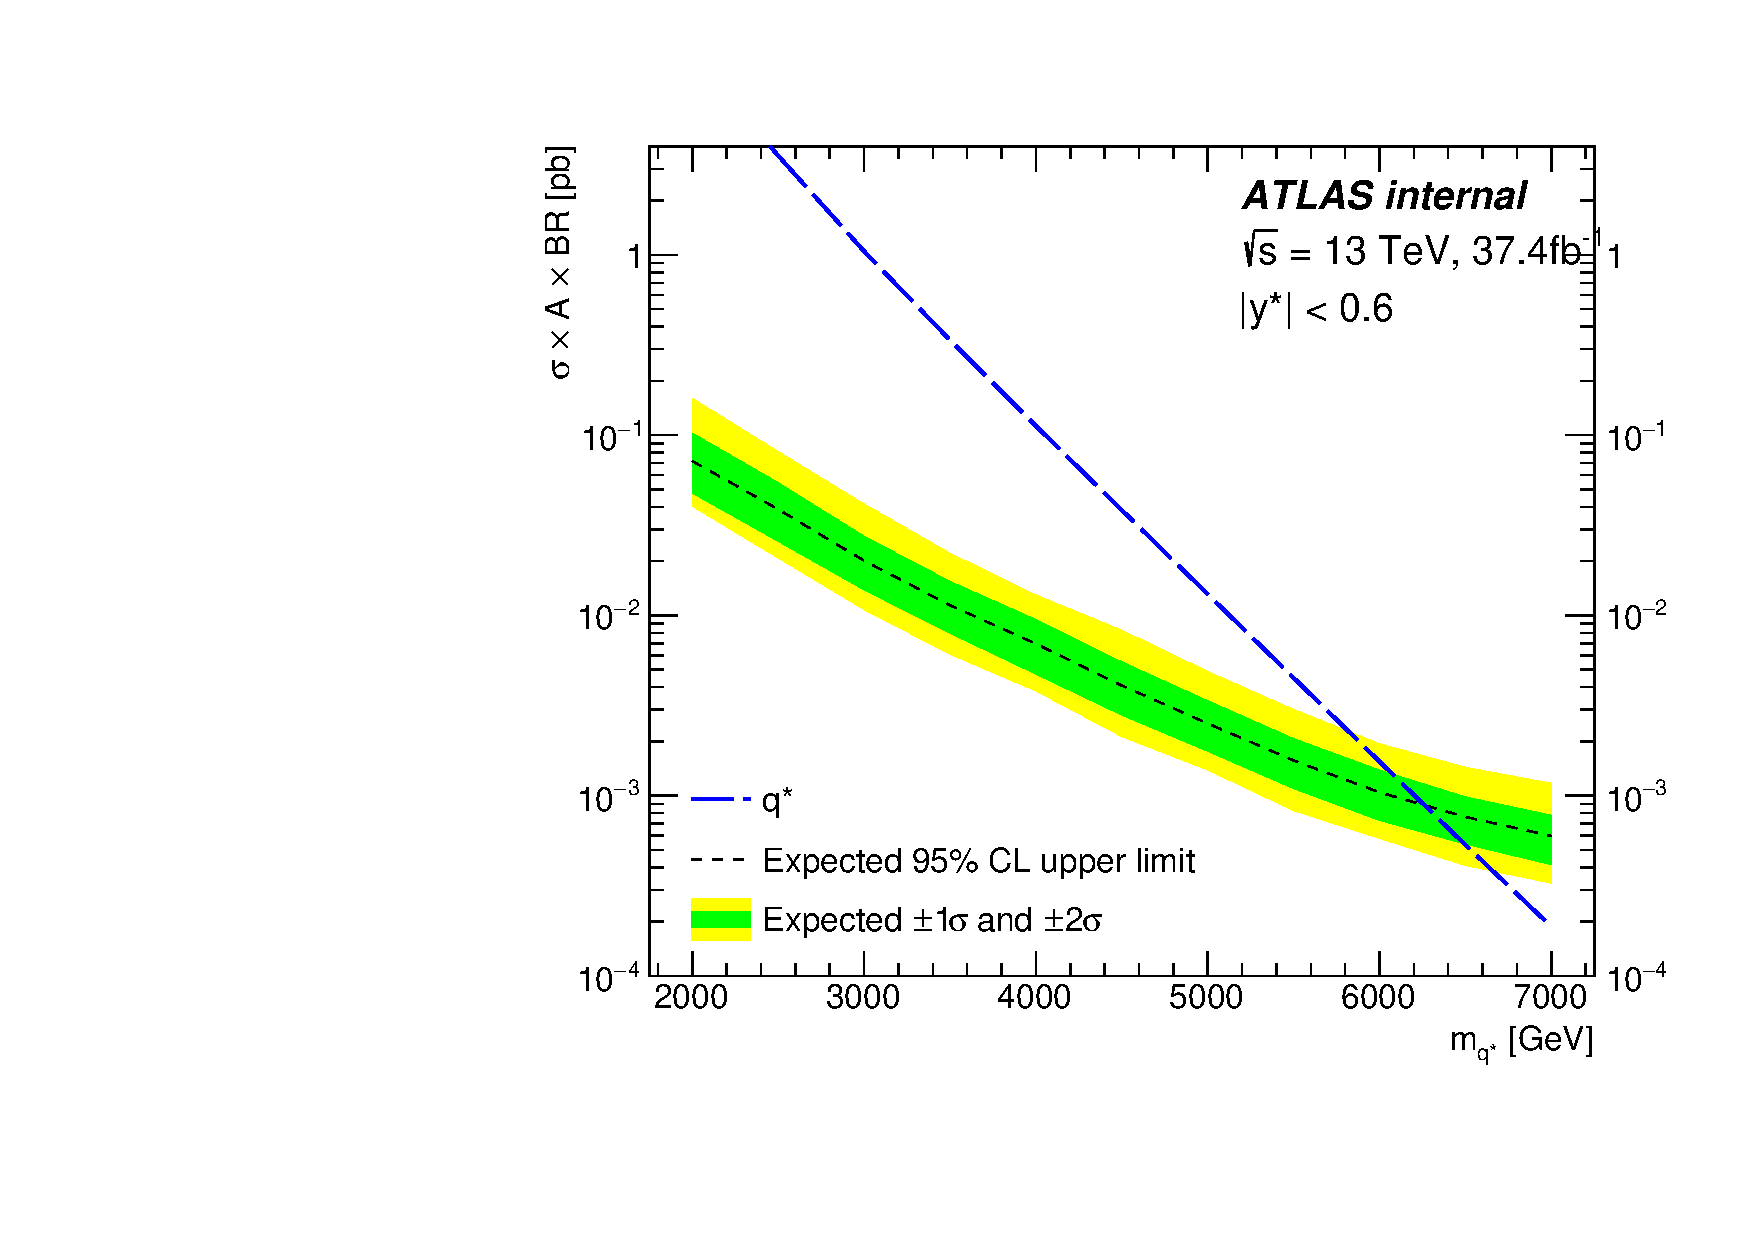
\includegraphics[width=0.475\textwidth] {figures/tagging/brazil-qStarMorphSingleCombinedUpdated.pdf}}
 \vspace*{-2mm}\\
 %
 \subfigure[\QQ] {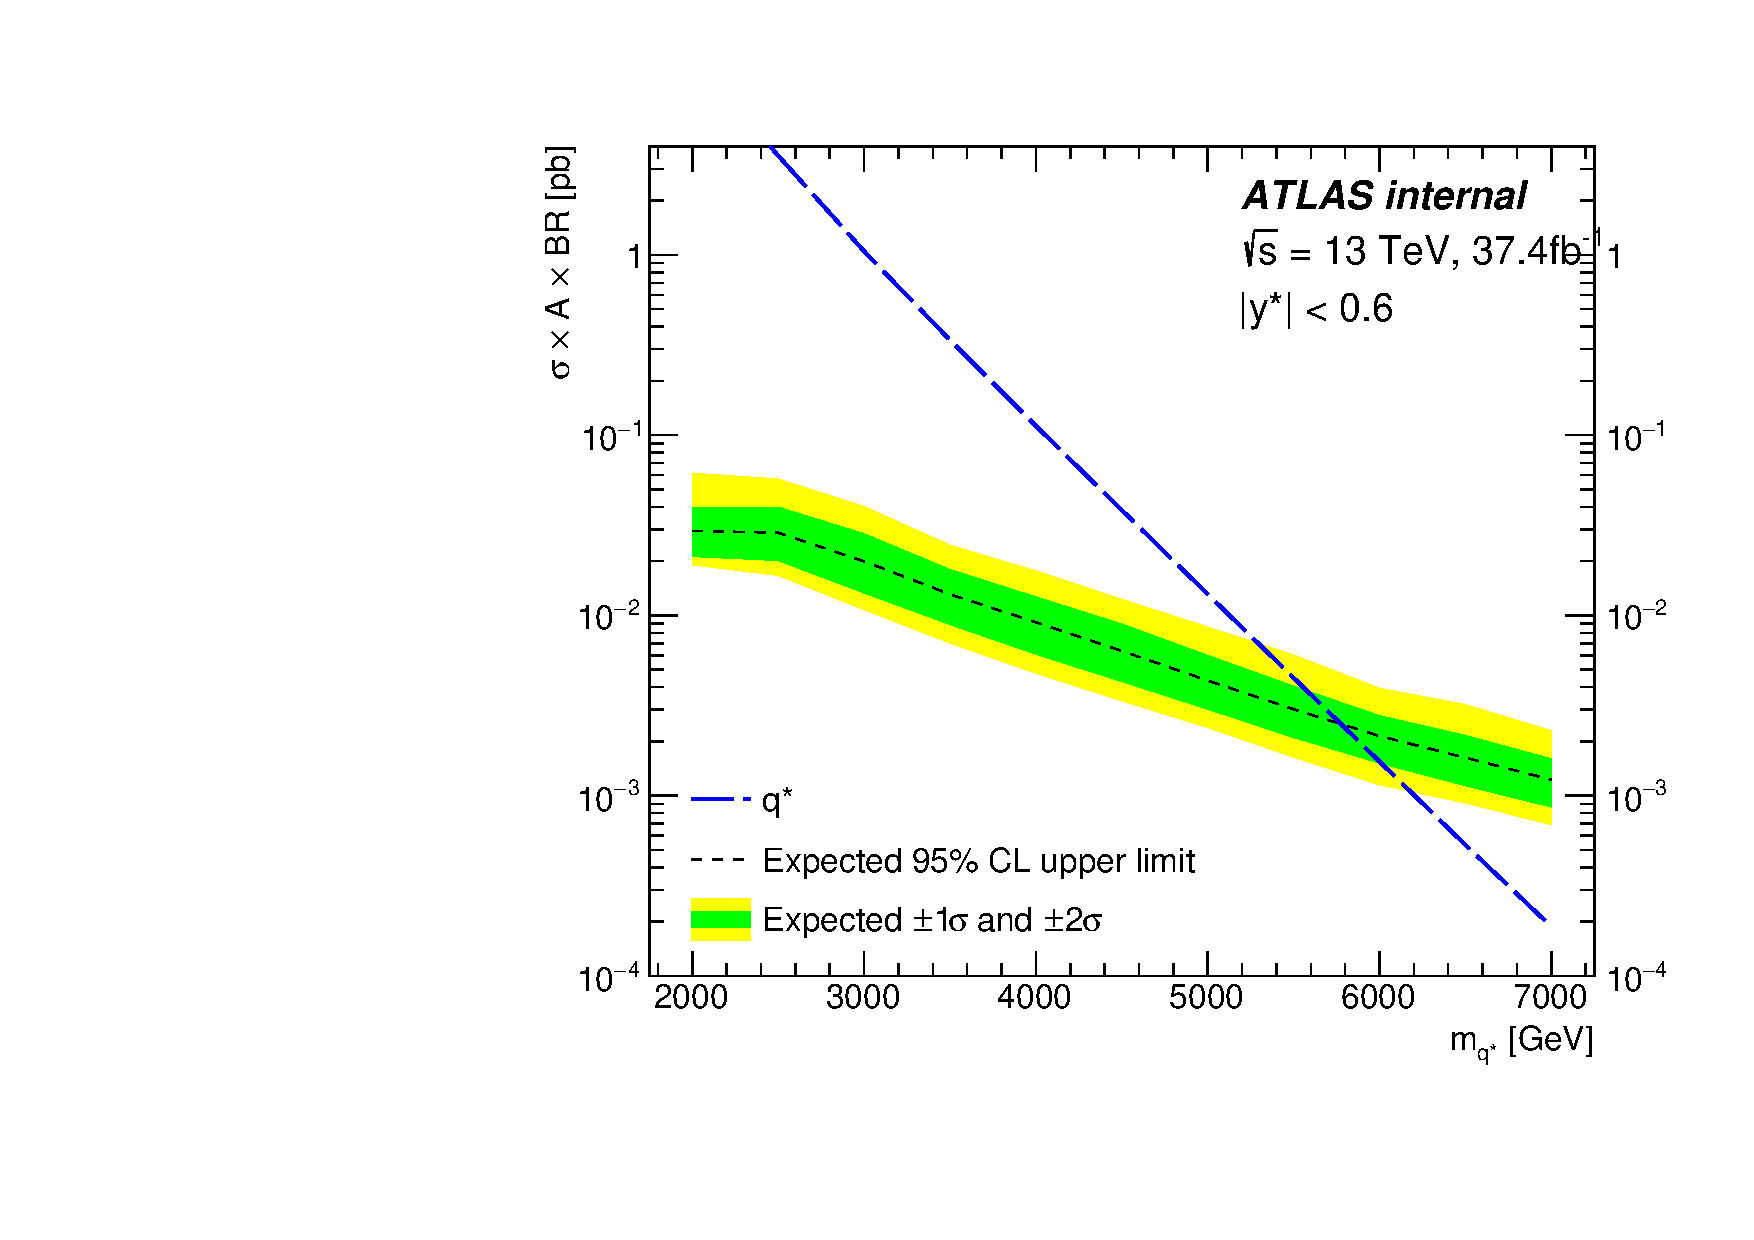
\includegraphics[width=0.475\textwidth] {figures/tagging/brazil-qStarMorphSingleQQUpdated}}
 \subfigure[\QG] {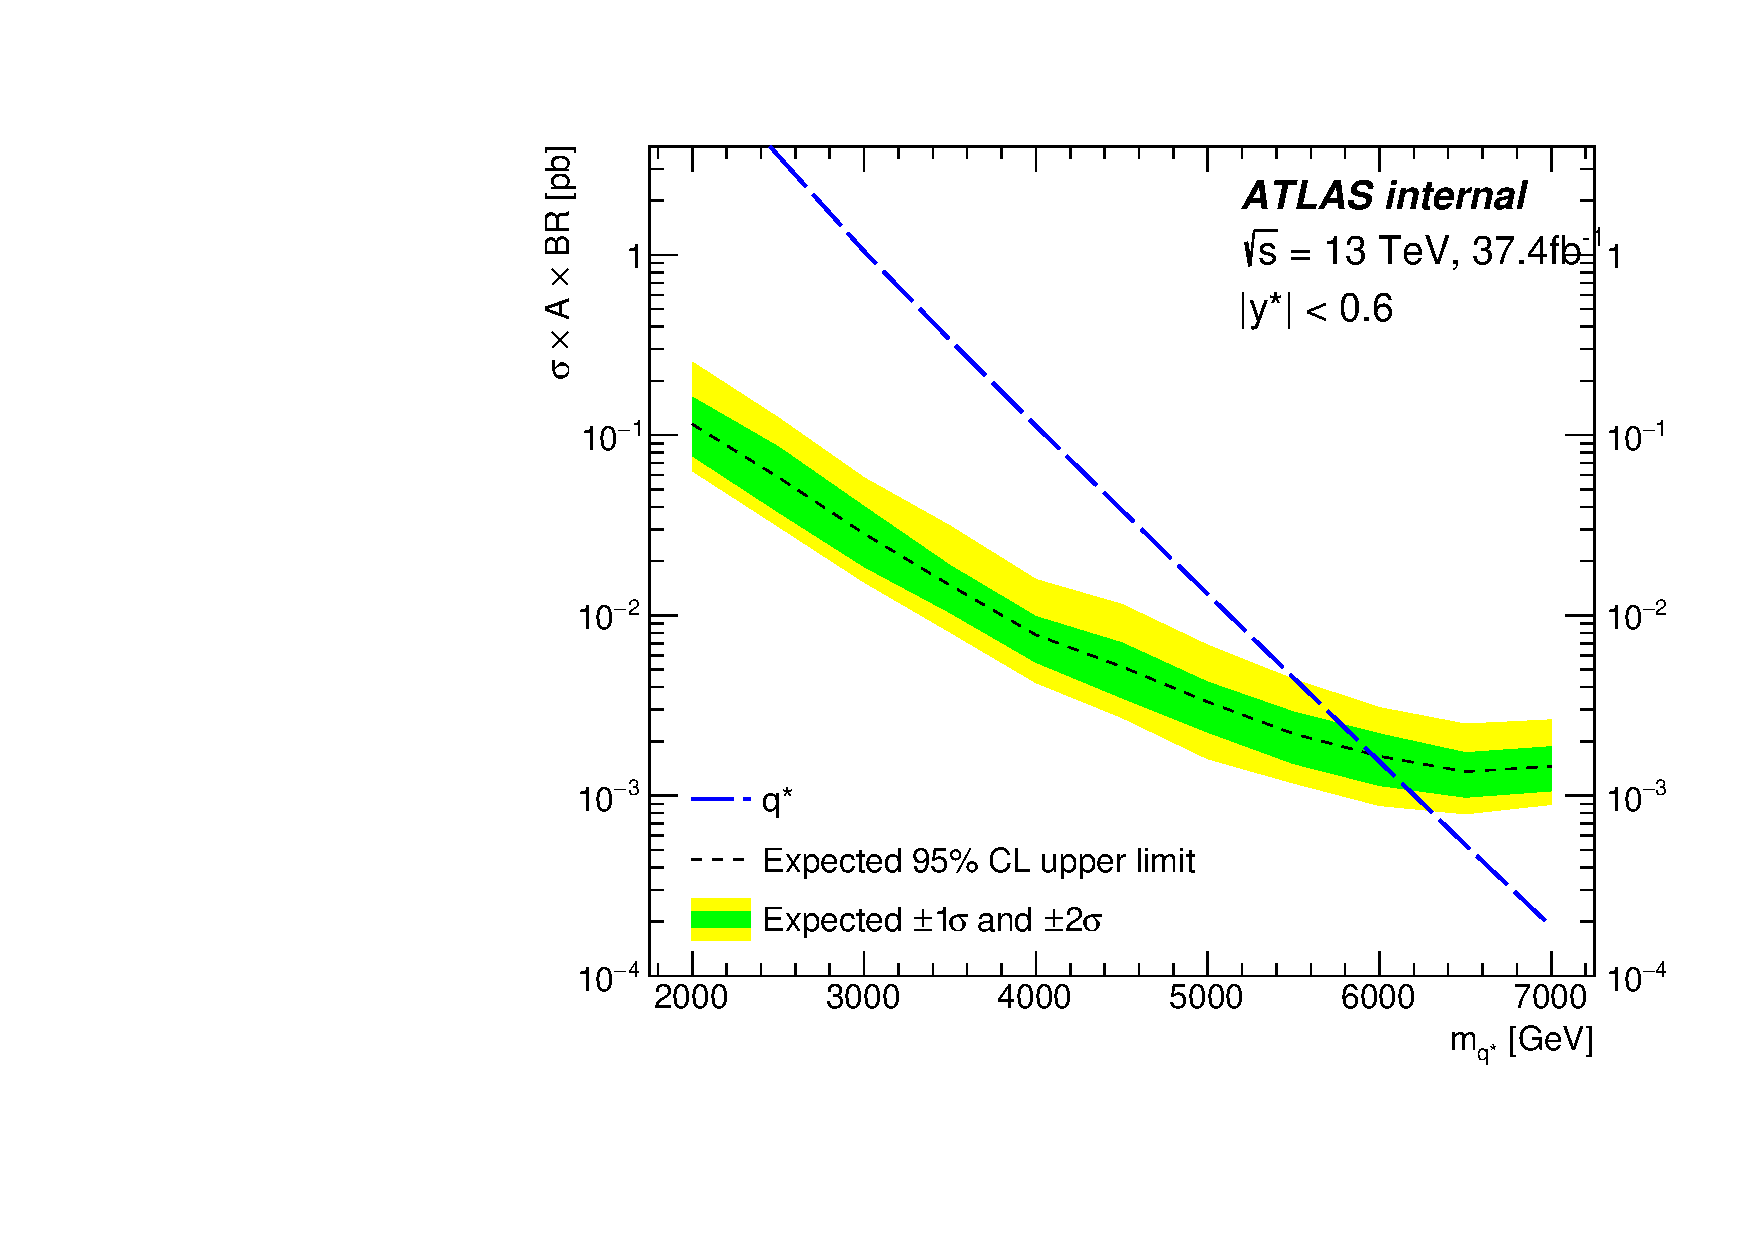
\includegraphics[width=0.475\textwidth] {figures/tagging/brazil-qStarMorphSingleQGUpdated}}
 \vspace*{-2mm}\\
 %
 \subfigure[\GG] {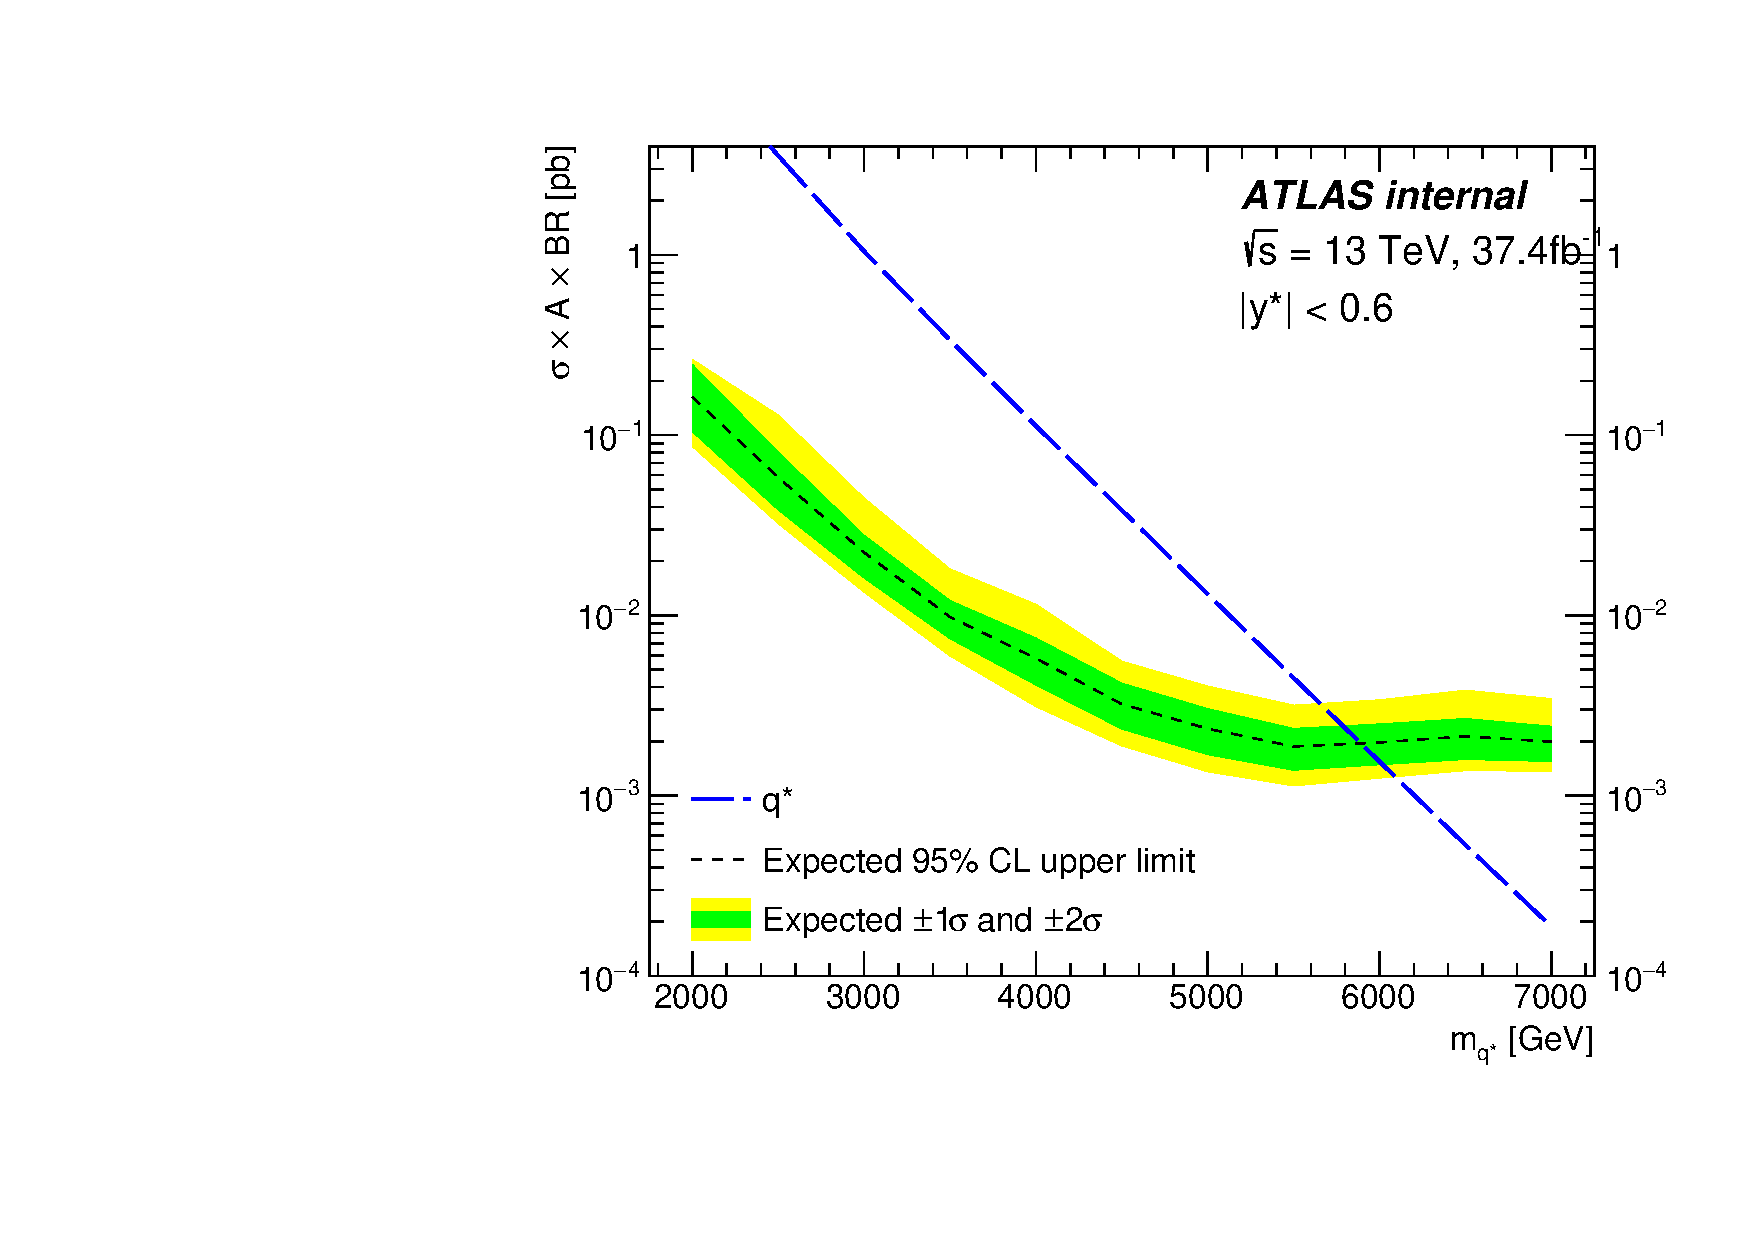
\includegraphics[width=0.475\textwidth] {figures/tagging/brazil-qStarMorphSingleGGUpdated}}
 \vspace*{-2mm}\\
 %

 \caption{Expected limits for a \qstar\ signal from  pseudo experiments for \integLumi\ for the 
 (a) \JJ\ resonant selection, (b) combined \QQ, \QG\ and \GG\ combined fit (c) \QQ\ sub-sample, (d) \QG\ sub-sample 
 and (e)  \GG\ sub-sample.
 \label{fig:toyMCExpectedLimitsqstar}}
\end{figure}





